% Method of the month: The Newey-West estimator and interrupted time series
% (c) 2021 Malcolm Gillies <malcolm.gillies@unsw.edu.au>
% https://github.com/mbg-unsw/neweywest
%
% This work is licensed under a
% Creative Commons Attribution-NonCommercial-ShareAlike 4.0
% International Licence
\documentclass[aspectratio=169,12pt]{beamer} % XXXX fix AR here
\usepackage[latin1]{inputenc}
\usepackage[T1]{fontenc}
\usepackage{textcomp}
\usefonttheme{serif} % need this with Charter font
\usetheme{Berlin}  % using default now
\usecolortheme{beaver}  % using default now
\usepackage[libertine]{libertine} % not using osf (old-style figures)
\usepackage[scale=0.9]{tgheros} % scale to match libertine
\usepackage[varqu,varl]{inconsolata}
\usepackage[libertine]{newtxmath}
\usepackage{graphicx}
\usepackage{tikz}
\usepackage{tikzpagenodes}
\usepackage{natbib}
\usepackage{gitinfo2}

\renewcommand{\gitMark}{\color{gray}\texttt{\tiny\gitBranch\,@\,\gitAbbrevHash\,\gitAuthorDate}}

\setbeamertemplate{navigation symbols}{} % remove navigation symbols
\setbeamercolor*{item}{fg=darkred}

\title{``Method of the month'': The Newey--West estimator and interrupted time series}
\author{Malcolm Gillies}
\date{20 May 2021}
\usebackgroundtemplate{%
\begin{tikzpicture}[remember picture,overlay]
    \node[anchor=south west,scale=1,rotate=90] at ([shift={(0cm,0cm)}]current page marginpar area.south east) {\gitMark};
\end{tikzpicture}%
}
\begin{document}

{
%\usebackgroundtemplate{}
\begin{frame}
\titlepage
\end{frame}
}

\begin{frame}{What is the Newey--West estimator?}
	\begin{itemize}
		\item Time series data are often \emph{autocorrelated}
		\item This messes up inference e.g. 95\% CI too small
		\item You can model the correlation structure e.g. ARIMA
		\item Or use a Heteroskedasticity- and Autocorrelation-Robust (aka HAC) method
		\begin{itemize}
			\item e.g. Newey--West (1987) or Newey--West (1994)
		\end{itemize}
	\end{itemize}
\end{frame}

\begin{frame}{How do I do use it?}
\texttt{library(sandwich)} \\
\texttt{library(lmtest)} \\
\medskip
\texttt{ts.lm <- lm(log(cnt)\textasciitilde 1+step+trend, data=tss)} \\
\texttt{coeftest(ts.lm2, df=Inf, vcov. = NeweyWest(ts.lm2, adjust=TRUE))}
\end{frame}

\begin{frame}{Is anyone else using it?}
	\begin{itemize}
		\item Review of ITS in healthcare
		\citep{hudson_methodology_2019}
		\begin{itemize}
			\item 2/116 studies published in 2015 used N--W
		\end{itemize}
		\item Review of ITS studies of public health interventions
		\citep{turner_design_2020}
		\begin{itemize}
			\item 2/200 studies publishd 2013--17 used N--W
		\end{itemize}
	\end{itemize}
\end{frame}

\usebackgroundtemplate{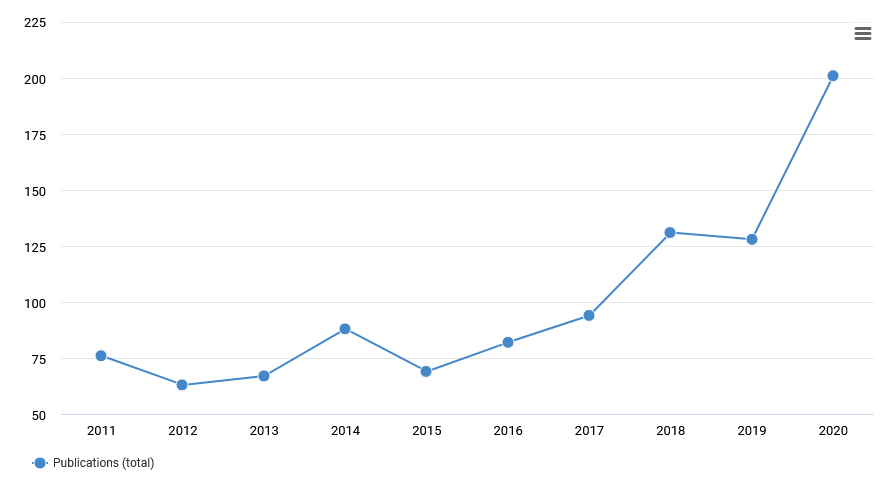
\includegraphics[width=\paperwidth]{ref/newey-west-cites.PNG}}
\begin{frame}[plain,b]
\begin{flushright}\texttt{https://app.dimensions.ai/}\end{flushright}
\end{frame}
\usebackgroundtemplate{}


\begin{frame}{Empirical comparison 1}
	\begin{itemize}
		\item Simulation study
		\citep{turner_evaluation_2020}
		\item Models fit with six methods:
		\begin{itemize}
			\item OLS, OLS/N--W, GLS/P--W, REML, REML/Satterthwaite, ARIMA
		\end{itemize}
		\item AR(1) data, N--W \texttt{lag=1}
		\item For inference \( T=48 \)
		\begin{itemize}
			\item ARIMA coverage OK
			\item REML similar to ARIMA, REML/Satterthwaite >100\% coverage
			\item \textbf{N--W poor coverage}
		\end{itemize}
	\end{itemize}
\end{frame}

\begin{frame}{Empirical comparison 2}
	\begin{itemize}
		\item Published ITS studies (\( n=190 \), median \(T=48\))
		\citep{turner_comparison_2020}
		\item Data re-fit with six methods:
		\begin{itemize}
			\item OLS, OLS/N--W, GLS/P--W, REML, REML/Satterthwaite, ARIMA
		\end{itemize}
		\item For inference
		\begin{itemize}
			\item REML/Satterthwaite most conservative
			\item ARIMA 2nd most conservative
			\item REML 3rd most conservative
		\end{itemize}
	\end{itemize}
\end{frame}

\begin{frame}{Bottom line}
    \begin{itemize}
        \item Don't use N--W (1987) with \texttt{lag=1}
        \item N--W (1994) with small sample adjustment might be OK
		\item AR(1) with REML estimation sounds good. How do we do it?
        \item Post-Newey--West methods tantalizingly close!
		\item Maybe stick with ARIMA after all?
    \end{itemize}
\end{frame}

\begin{frame}{What do the econometricians say?}
HAR Inference: Recommendations for Practice

\cite{lazarus_har_2018}
\end{frame}

\begin{frame}{Thanks}
    \begin{itemize}
        \item Andrea
    \end{itemize}
\end{frame}

\begin{frame}{References}
%        \bibliographystyle{apalike}
%        \bibliographystyle{abbrv}
        \tiny\bibliography{nw.bib}
        \bibliographystyle{abbrvnat}
\end{frame}

\end{document}
